% !TEX TS-program = pdflatex

\documentclass[unicode,11pt,notheorems,xcolor=table]{beamer}

\usepackage[T2A]{fontenc}
\usepackage[utf8]{inputenc}
\usepackage[russian]{babel}
\usepackage{amsmath,amsfonts,amssymb,amsthm}
\usepackage{mathtools}
\usepackage{diagbox}

\usepackage{ulem}
\usepackage{tikz, graphicx}
%\usepackage{tkz-graph}
\usetikzlibrary{matrix,arrows,decorations.pathmorphing, arrows.meta,positioning}
\usetikzlibrary{positioning,calc}
\usetikzlibrary{petri}
\usetikzlibrary{decorations.pathreplacing}

%Описание стиля презентации
\usetheme[sidebar=0]{kfmn} 
\setbeamercovered{transparent}

%\definecolor{cyan}{RGB}{240,217,1}
%\definecolor{vgugreen}{RGB}{143,188,103}
%\definecolor{vgured}{RGB}{234,38,40}
%\definecolor{vgublue}{RGB}{53,101,167}



\makeatletter
	\g@addto@macro{\endtabular}{\rowfont{}}% Clear row font
	\makeatother
	\newcommand{\rowfonttype}{}% Current row font
	\newcommand{\rowfont}[1]{% Set current row font
		\gdef\rowfonttype{#1}#1\ignorespaces%
	}
\makeatother

\newcommand{\myunit}{9mm}
\tikzset{
    node style sp/.style={draw,circle,minimum size=\myunit},
    node style ge/.style={circle,minimum size=\myunit},
    arrow style mul/.style={draw,sloped,midway,fill=white},
    arrow style plus/.style={midway,sloped,fill=white},
}

%[0, 6, 8, 8, 10, 5, 6, 10, 8, 10, 10], 

\pgfdeclareimage[height=8mm]{university-logo}{logo-iem.png}
\logo{\pgfuseimage{university-logo}}
%2[0, 11, 10, 8, 11, 5, 11, 11, 8, 11, 10, 11],

\titlepicture{
	\begin{tikzpicture}[y=1.4cm,overlay,rotate=8]
	\coordinate (O) at (-3cm,0.9cm);
	\filldraw[thick,draw= vgublue, fill=vgublue!20!white] (0,0) circle[radius=4.2cm];
	\clip (0,0) circle[radius=4.2cm];
	\draw (-1.5,1.5) node{
	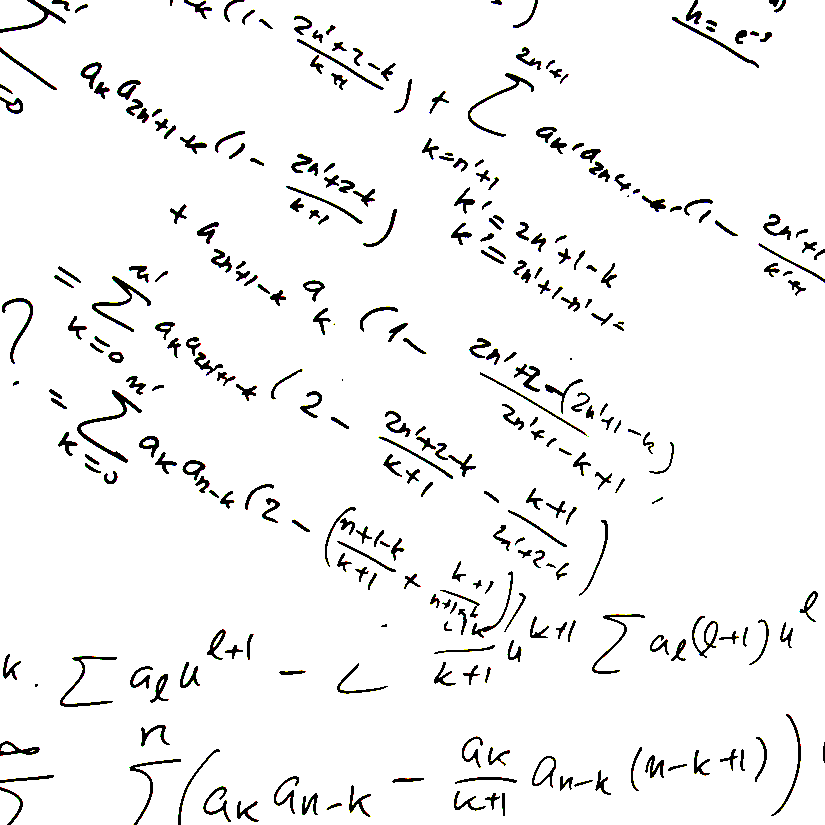
\includegraphics[width=8cm]{titlepic.png}
	};
\end{tikzpicture}
}

\usepackage[math]{iwona}

\newcommand{\hplus}{\mathbin{\hat+}}
\newcommand{\hdot}{\mathbin{\hat\cdot}}
% Описание теорем
\newtheorem{theorem}{Теорема}
\newtheorem{seq}{Следствие}
%%

%\VKR
\LECT % можно ещё лекцию забацать.
%\REPORT % можно ещё лекцию забацать.

%\titlepicture{
%%	\begin{tikzpicture}[overlay]
%%			\draw[opacity=0.4]  (-0.3,1.8) node {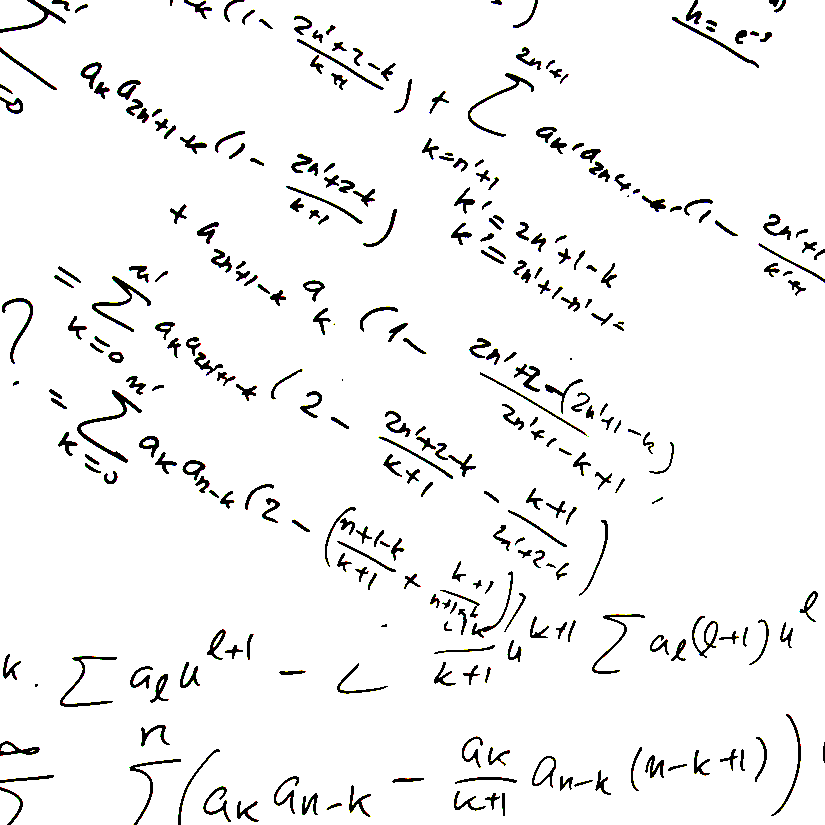
\includegraphics[width=3.5cm]{titlepic.png}};
%%	\end{tikzpicture}
%}

% Титульный лист теорем
\author[Д.\,В. Чупраков]{канд.\,физ.-матем.\,наук, доцент Д.\,В. Чупраков\\[6pt] usr10381@vyatsu.ru}

\institute[ВятГУ]{ФГБОУ ВО Вятский государственный университет}

\department{Факультет экономики и финансов}

\title[Лекция~7. Динамическое программирование]{
	Введение в экономико-математическое моделирование\\[12pt]
	Лекция~7. Динамическое программирование}
%\subtitle{Теория двойственности и транспортная задача}

\date{19 октября 2020~г.}


%\setbeamercolor{coloredboxstuff}{fg=yellow,bg=white!10!blue}

\setbeamercovered{invisible}


%\tikzset{
%	 myarrow/.style={->, >=latex', shorten >=1pt, thick}
%}
%
%
%
%\tikzset{add/.style n args={4}{
%    minimum width=6mm,
%    path picture={
%        \draw[black] 
%            (path picture bounding box.south east) -- (path picture bounding box.north west)
%            (path picture bounding box.south west) -- (path picture bounding box.north east);
%        \node at ($(path picture bounding box.south)+(0,0.13)$)     {\tiny #1};
%        \node at ($(path picture bounding box.west)+(0.13,0)$)      {\tiny #2};
%        \node at ($(path picture bounding box.north)+(0,-0.13)$)        {\tiny #3};
%        \node at ($(path picture bounding box.east)+(-0.13,0)$)     {\tiny #4};
%        }
%    }
%}
%
%\tikzset{bigadd/.style n args={4}{
%    minimum width=20mm,
%    path picture={
%        \draw[black] 
%            (path picture bounding box.south east) -- (path picture bounding box.north west)
%            (path picture bounding box.south west) -- (path picture bounding box.north east);
%        \node at ($(path picture bounding box.south)+(0,0.5)$)     { #1};
%        \node at ($(path picture bounding box.west)+(0.5,0)$)      {#2};
%        \node at ($(path picture bounding box.north)+(0,-0.5)$)        {#3};
%        \node at ($(path picture bounding box.east)+(-0.5,0)$)     {#4};
%        }
%    }
%}



\begin{document}


\maketitle

\begin{frame}{Структура лекции}
	\tableofcontents
\end{frame}



\section{Динамическое программирование}
\begin{frame}{Динамическое программирование}{}

	\alert{Динамическое программирование}~--- это метод нахождения оптимальных решений в задачах с \alert{многоэтапной структурой}. 


	\medskip
	
	Многие экономические процессы расчленяются на шаги естественным образом. Это все процессы планирования и управления, развивающиеся во времени.
	\begin{itemize}
		\item из года в год меняется возраст машин и оборудования;
		\item трудозатраты меняются от работы к работе в рамках сетевой модели;
		\item руководство предприятием требует принятия решений в зависимости от свершившихся событий. 
	\end{itemize}

 	Очевидно, в таких задачах необходимо принимать оптимальные решения не только на текущий момент,  но и на весь рассматриваемый период в целом с учетом возможных изменений параметров. 
 
	\medskip
     ДП связано с именем Ричарда Беллмана, который сформулировал принцип, позволяющий существенно сократить перебор решений в многоэтапных нелинейных задачах. 
\end{frame}



\section{Постановка задачи динамического программирования}

\begin{frame}{Управляемая система без памяти}{}

\begin{itemize}
%\item 
%	\structure{Управляемый процесс}
%	\begin{itemize}
%	\item 
%		процесс распределения средств между предприятиями,
%	\item 
%		распределения ресурсов в течение ряда лет
%	\end{itemize}

\item \structure{Конечность числа шагов:}\\
	В результате управления система~$S$ переводится из начального состояния~$S_0$  в~состояние~$S_n$. 

\item 
	На каждом шаге  $k = \{1,2,\ldots, n\}$ принимается допустимое управляющее решение~$x_k$.


%Переменные  $x_k$  удовлетворяют некоторым ограничениям и в этом смысле называются допустимыми.

%Предположим, что управление можно разбить на  $n$  шагов, т.е.
%решение принимается последовательно на каждом шаге, а управление, переводящее систему из  $S_0$  в  $\hat S$, можно
%представить в виде последовательности  $n$  пошаговых управлений.

%Пусть 

\item \structure{Система без памяти:} 		$S_k=\varphi(S_{k-1},x_k)$

%	$S_k$~--- состояние системы после $k$-го шага управления.
		Состояние системы $S_k$ в конце $k$-го шага определяется:
		\begin{itemize}
		\item 
			предшествующим состоянием $S_{k-1}$
		\item 
		 	управлением~$x_k$ 
		\item 
		 	 \alert{не~зависит от других состояний и~управлений}		
		 \end{itemize}

\end{itemize}

\bigskip
\structure{Управляемая система:}
$S_0 \xrightarrow{x_1} S_1\xrightarrow{x_2} S_2 \xrightarrow{x_3}\ldots\xrightarrow{x_{n-1}} S_{n-1} \xrightarrow{x_n} \alert{S_n}.
$

\smallskip
\structure{Управление:}\hspace{16mm} $X = (x_1,x_2,\ldots,x_{n-1},x_n)$
\end{frame}

\begin{frame}{Постановка задачи ДП}

\structure{Показатель эффективности управления}~--- целевая функция
$$
	F = F(S_0,X)
$$



Предположим, $F$ имеет \alert{свойство аддитивности}:
$$
		F=\sum_{k=1}^n f_k(S_{k-1},x_k) = f_1(S_0,x_1)+f_2(S_1,x_2)+\ldots+ f_n(S_{n-1},x_n)
$$
$f_k$ --- показатель эффективности управления на~$k$-м шаге.

\bigskip

\begin{block}{Общая формулировка задачи динамического программирования}
	Определить такое допустимое управление $X = (x_1,x_2,\ldots,x_{n-1},x_n)$, переводящее систему  $S$  из~состояния~$S_0$  в состояние~$S_n$, при котором целевая функция~$F=F(S_0,X)$ принимает наибольшее значение.
\end{block}
\end{frame}

\begin{frame}{Особенности модели ДП}{}
\begin{enumerate}
\item 
	Задача оптимизации интерпретируется как $n$-шаговый процесс управления.
\item 
	Целевая функция (ЦФ)~--- сумма ЦФ на каждом шаге.
\item 
	Выбор управления на $k$-ом шаге зависит только от состояния системы к этому шагу и не влияет на предшествующие шаги (нет обратной связи).
\item 
	Состояние системы после $k$-го шага управления зависит от предшествующего состояния и управления.
\item 
	На каждом шаге управление~$x_k$  зависит от конечного числа управляющих переменных, а состояние  $S_k$ --- от конечного числа параметров.
\end{enumerate}
\end{frame}


\section{Принцип оптимальности Беллмана}

\begin{frame}{Принцип оптимальности Беллмана}
%\begin{itemize}
%\item 
%	Нас интересует результат управления в целом за все шаги.
%\item 
%	Принимая решение на отдельном этапе, мы должны выбирать оптимальное управляющее  воздействие ,,с прицелом на будущее``.
%\end{itemize}
%

\begin{alertblock}{Вопрос:}
 Что такое оптимальность управления на $k$-м  шаге?
\end{alertblock}
	
\bigskip
    \alert{Условный оптимальный выигрыш~$W_k(S)$}~--- величина выигрыша от $k$-го шага и до конца, если $k$-ый шаг начинается с некоторого состояния $S$.
	$$
		F_k(S_{k-1})
		%=\sum_{i=k}^n f_i(S_{i},x_{i+1}) 
		= f_{k}(S_{k-1},x_{k})+f_{k+1}(S_{k},x_{k+1})+\ldots+ f_n(S_{n-1},x_n)
	$$
	
       
	\begin{block}{Принцип оптимальности Беллмана} 
		Принимая решение $k$-ом шаге, нужно выбрать управление~$x_k$ так, чтобы условный оптимальный выигрыш $F_k(S_{k-1})$ был~максимальным. 
	\end{block}

\structure {Ограничение:} 
\alert{Управление на данном шаге не должно оказывать влияние на предшествующие шаги.}

\end{frame}

%\begin{frame}{}
%Принцип оптимальности утверждает, что для любого процесса без обратной связи оптимальное управление таково, что является
%оптимальным для любого подпроцесса по отношению к его исходному состоянию. Поэтому решение на каждом шаге оказывается наилучшим с точки зрения управления в целом.
%
%
%Рассмотрим вместо исходной задачи ДП с фиксированным числом шагов  $n$  и начальным состоянием  $S_0$ 
%последовательность задач, полагая  $n=1,\;2,\ldots $  при различных  $S$  одношаговую, двухшаговую и т.д., используя
%принцип оптимальности.
%
%На каждом шаге любого состояния  $S_{k-1}$  решение  $X_k$  влияет на последующее состояние $S_k$.
%
%\end{frame}


\begin{frame}{Последний шаг управления}

%Рассмотрим   $n$-й шаг:

{\small
\begin{itemize}
\item 
	$S_{n-1}$~--- состояние системы к началу $n$-го шага;
\item 
	$S_n$~--- конечное состояние;
\item 
	$X_n=x_n$~--- допустимое управляющее воздействие;
\item 
	$f_n (S_{n-1},x_n)$~--- целевая функция $n$-го шага.
\end{itemize}\par}


\structure{По принципу оптимальности} \alert{$F_n(S_{n-1},X_n) = f_n(S_{n-1},x_n) \to \max$}.

\begin{itemize}
\item 
\alert{$F_n^*(S_{n-1})$}~--- максимум целевой функции $n$-го шага если система была в состоянии $S_{n-1}$.
$$
F_n^*(S_{n-1}) = \max_{x_n} \big\{f_n(S_{n-1},x_n) \big\}
$$

\item 
 \alert{$x_n^*\left(S_{n-1}\right)$}~--- \alert{условно оптимальное управление на 
 $n$-ом шаге}~--- решение  $x_n$, при котором достигается  $F_n^*\left(S_{n-1}\right)$.
\end{itemize}

\begin{block}{}
Решив задачу нахождения максимума функции одной переменной $x_n$ найдем $F_n^*\left(S_{n-1}\right)$  и $x_n^*(S_{n-1})$.
\end{block}

\end{frame}

\begin{frame}{Предпоследний шаг управления}

\structure{В силу аддитивности}
$$
	\alert{F_{n-1}(S_{n-2},X_{n-1})=f_{n-1}(S_{n-2},x_{n-1})+F^*(S_{n-1})}
$$

для $X_{n-1}=(x_{n-1},x_n^*)$, где $x_n^*$~--- оптимальное управление $n$-го шага.  

\structure{По принципу оптимальности} $F_{n-1}(S_{n-2})\to \max$.



\begin{multline*}
	F_{n-1}^*(S_{n-2}) 
	= \max_{x_{n-1}} \{f_{n-1}(s_{n-2},x_{n-1})+ F_n^*(S_{n-1})\}
	=\\
	= \max_{x_{n-1}} \Big\{f_{n-1}(S_{n-2},x_{n-1})+ F_n^*\big(\varphi (S_{n-2},x_{n-1})\big)\Big\}
\end{multline*}

т.\,к.  $S_{n-1}=\varphi (S_{n-2},x_{n-1})$.

\begin{block}{}
Решив задачу нахождения максимума функции одной переменной $x_{n-1}$ 
найдем 

{\centering $F_n^*\left(S_{n-1}\right)$\quad и\quad $X_{n-1}^*=(x_{n-1}^*(S_{n-2}),x_n^*(S_{n-1}))$.\par}
\end{block}

\end{frame}

\begin{frame}{Рекуррентное соотношение Беллмана}{}
$F_k^*(S_{k-1})$~--- условный максимум целевой функции, полученной на  $n-k+1$  шагах, начиная с  $k$-го  до конца

\begin{block}{Основное рекуррентное соотношение Беллмана}
 \begin{align*}
 F_k^*(S_{k-1}) &=\max_{x_k} \big\{f_k(s_{k-1},x_k)+F_{k+1}^*(S_k) \big\}\\
 F_{k+1}(S_k) &= \max_{x_i} \sum_{i=k+1}^n f_i(S_{i-1},x_i)\\
 S_k &= \varphi (S_{k-1},x_k)
 \end{align*}
\end{block}
% $x_k$ {}- условно оптимальное управление на  $k-$ том шаге. Чтобы его найти, необходимо вместо  $S_k$  подставить 
%$$.

%Управление  $x_k$ {}- называется условно-оптимальным управлением на  $k-\text{\textcyrillic{м}}$  шаге.
%

%Условный максимум целевой функции за n шагов:
%
% $F_{\text{max}}=F_1^0\left(S_0\right)$.
%
%Далее, используя последовательность условных оптимальных управлений и уравнение состояния, находим оптимальное решение
%задачи ДП.

\end{frame}



























\begin{frame}{Схема применения метода ДП}{}


\begin{enumerate}
\item 
	Рассматриваем последний шаг и находим условный максимум целевой функции для каждого $S_{n-1}$
	$$
		\alert{F_n^*(S_{n-1})= \max_{x_n} \big\{f_n(s_{n-1},x_n) \big\} }
	$$
\item
	Двигаясь с конца, для каждого~$k$  находим условные максимумы целевой функции за  $n-k+1$  шагов, начиная с  $k$-го до конца по всем возможным управлениям~$x_k$:
	$$
		\alert{F_k^* (S_{k-1}) = \max_{x_k}  \big\{f_k(S_{k-1}, x_k) + F_{k+1}^*(S_k, x_{k+1}) \big\},}
%\quad k = n-1,\;n-2,\;\ldots,\;2,\;1
$$

%где:  $F_{k+1}^*\left(S_k,x_{k+1}\right)=F_{k+1}^*\left(S_k\right)=\underset{x_i}{\text{max}}\left\{\overset
%n{\underset{i=k+1}{\sum }}f_i\left(S_{i-1},x_i\right)\right\}.$  

Получаем последовательности условных оптимумов и условно оптимальных решений соответственно:
$$
\begin{array}{ccccc}
F_n^*(S_{n-1}) & F_{n-1}^*(S_{n-2})& \cdots & F_2^*(S_1) & F_1^*(S_0)\\
x_n^*(S_{n-1}) & x_{n-1}^*(S_{n-2})& \cdots & x_2^*(S_1) & x_1^*(S_0)\\
\end{array}
$$

\item 
	Искомый оптимум целевой функции~--- \alert{$F_1^*(S_0)$};
	
	оптимальное решение~---  \alert{$X^*=(x_1^*, x_{2}^*, \ldots, x_{n}^*)$.}
\end{enumerate}

\end{frame}





\section{Некоторые задачи}

\begin{frame}{}{}
\centering
\bfseries
\LARGE \color{vgublue} Некоторые задачи,\\ решаемые методом\\ динамического программирования
\end{frame}
\begin{frame}{Поиск оптимального маршрута}{}
\begin{exampleblock}{}
Прокладывается участок дороги из пункта~$A$ в пункт~$B$ по пересеченной местности. 
Требуется провести дорогу, чтобы суммарные затраты на сооружение участка были минимальные. 
\end{exampleblock}

\structure{Формализация:}
\begin{itemize}
\item
	Участок местности разбивается на сеть узлов.
\item
	Узлы соединяются дугами, веса $w_i$ которых обозначают затраты на строительство данного куска дороги.
\item
	Требуется в полученном графе найти путь наименьшей стоимости. 
	$$
	W= \sum w_i \to \min 
	$$
\end{itemize}
\end{frame}

\begin{frame}{Поиск оптимального маршрута. Граф}{}
\centering
\begin{tikzpicture}[
		baseline,
		>=latex,
	]
	\foreach \x in {1,2,...,6}
		\foreach \y in {1,2,...,6}
			\coordinate (n-\x-\y) at (1.8*\x,1.4*\y);
	\draw[above] 
		(n-1-1)--node{10} (n-2-1)--node{6} (n-3-1)--node{8} (n-4-1)--node{12} (n-5-1) --node{10} (n-6-1)
		(n-1-2)--node{9} (n-2-2)--node{11} (n-3-2)--node{9} (n-4-2)--node{7} (n-5-2) --node{9} (n-6-2)
		(n-1-3)--node{9} (n-2-3)--node{12} (n-3-3)--node{8} (n-4-3)--node{11} (n-5-3) --node{9} (n-6-3)
		(n-1-4)--node{6} (n-2-4)--node{10} (n-3-4)--node{11} (n-4-4)--node{6} (n-5-4) --node{14} (n-6-4)
		(n-1-5)--node{7} (n-2-5)--node{13} (n-3-5)--node{9} (n-4-5)--node{12} (n-5-5) --node{9} (n-6-5)		
		(n-1-6)--node{9} (n-2-6)--node{8} (n-3-6)--node{9} (n-4-6)--node{10} (n-5-6) --node{9} (n-6-6)
	;
	\draw[right] 
		(n-1-1)--node{10} (n-1-2)--node{9} (n-1-3)--node{8} (n-1-4)--node{6} (n-1-5) --node{7} (n-1-6)
		(n-2-1)--node{11} (n-2-2)--node{10} (n-2-3)--node{9} (n-2-4)--node{6} (n-2-5) --node{6} (n-2-6)
		(n-3-1)--node{10} (n-3-2)--node{9} (n-3-3)--node{8} (n-3-4)--node{9} (n-3-5) --node{8} (n-3-6)
		(n-4-1)--node{8} (n-4-2)--node{5} (n-4-3)--node{9} (n-4-4)--node{6} (n-4-5) --node{7} (n-4-6)
		(n-5-1)--node{10} (n-5-2)--node{6} (n-5-3)--node{9} (n-5-4)--node{10} (n-5-5) --node{7} (n-5-6)
		(n-6-1)--node{11} (n-6-2)--node{9} (n-6-3)--node{5} (n-6-4)--node{12} (n-6-5) --node{8} (n-6-6)
	;
	\foreach \x in {1,2,...,6}
		\foreach \y in {1,2,...,6}
		{
			\node [
				fill=vgublue!30,
				minimum height=5mm,
				minimum width=8mm
			] 
			at (n-\x-\y) {~};	
		}
	\begin{scope}[
		every node/.style={
			fill=vgured!30,
			minimum height=5mm,
			minimum width=8mm
		}
	] 
		\node at (n-1-1) {$A$};
		\node at (n-6-6) {$B$};
	\end{scope}
\end{tikzpicture}
\end{frame}


\begin{frame}{Поиск оптимального маршрута. Решение}{}
\centering
\begin{tikzpicture}[
		baseline,
		>=latex,
	]
	\foreach \x in {1,2,...,6}
		\foreach \y in {1,2,...,6}
			\coordinate (n-\x-\y) at (1.7*\x,1.3*\y);
	\draw[above] 
		(n-1-1)--node{10} (n-2-1)--node{6} (n-3-1)--node{8} (n-4-1)--node{12} (n-5-1) --node{10} (n-6-1)
		(n-1-2)--node{9} (n-2-2)--node{11} (n-3-2)--node{9} (n-4-2)--node{7} (n-5-2) --node{9} (n-6-2)
		(n-1-3)--node{9} (n-2-3)--node{12} (n-3-3)--node{8} (n-4-3)--node{11} (n-5-3) --node{9} (n-6-3)
		(n-1-4)--node{6} (n-2-4)--node{10} (n-3-4)--node{11} (n-4-4)--node{6} (n-5-4) --node{14} (n-6-4)
		(n-1-5)--node{7} (n-2-5)--node{13} (n-3-5)--node{9} (n-4-5)--node{12} (n-5-5) --node{9} (n-6-5)		
		(n-1-6)--node{9} (n-2-6)--node{8} (n-3-6)--node{9} (n-4-6)--node{10} (n-5-6) --node{9} (n-6-6)
	;
	\draw[right] 
		(n-1-1)--node{10} (n-1-2)--node{9} (n-1-3)--node{8} (n-1-4)--node{6} (n-1-5) --node{7} (n-1-6)
		(n-2-1)--node{11} (n-2-2)--node{10} (n-2-3)--node{9} (n-2-4)--node{6} (n-2-5) --node{6} (n-2-6)
		(n-3-1)--node{10} (n-3-2)--node{9} (n-3-3)--node{8} (n-3-4)--node{9} (n-3-5) --node{8} (n-3-6)
		(n-4-1)--node{8} (n-4-2)--node{5} (n-4-3)--node{9} (n-4-4)--node{6} (n-4-5) --node{7} (n-4-6)
		(n-5-1)--node{10} (n-5-2)--node{6} (n-5-3)--node{9} (n-5-4)--node{10} (n-5-5) --node{7} (n-5-6)
		(n-6-1)--node{11} (n-6-2)--node{9} (n-6-3)--node{5} (n-6-4)--node{12} (n-6-5) --node{8} (n-6-6)
	;
	\foreach \x in {1,2,...,6}
		\foreach \y in {1,2,...,6}
		{
			\node [
				fill=vgublue!30,
				minimum height=5mm,
				minimum width=8mm
			] 
			at (n-\x-\y) {~};	
		}
		
	\begin{scope}[line width=2pt, vgublue]
%			\only<2>{\draw (n-6-5)--(n-6-6);}
%			\only<3>{\draw (n-5-5)--(n-5-6)--(n-6-6);}
%			\only<4>{\draw (n-6-3)--(n-6-4)--(n-6-5)--(n-6-6);}
%			\only<5>{\draw (n-4-4)--(n-5-4)--(n-5-5)--(n-6-5)--(n-6-6);}
%			\only<6>{\draw (n-5-2)--(n-5-3)--(n-6-3)--(n-6-4)--(n-6-5)--(n-6-6);}
%			\only<7>{\draw (n-4-2)--(n-4-3)--(n-4-4)--(n-5-4)--(n-5-5)--(n-5-6)--(n-6-6);}
%			\only<8>{\draw 
%				(n-4-1)--(n-4-2)--(n-4-3)--(n-4-4) --
%				(n-5-4)--(n-5-5)--(n-5-6)--(n-6-6);
%			}
%			\only<9>{\draw 
%				(n-3-1)--(n-4-1)--(n-4-2)--(n-4-3)--(n-4-4) --
%				(n-5-4)--(n-5-5)--(n-5-6)--(n-6-6);
%			}
%			\only<10>{\draw 
%				(n-2-1)--(n-3-1)--(n-4-1)--(n-4-2)--(n-4-3)--(n-4-4) --
%				(n-5-4)--(n-5-5)--(n-5-6)--(n-6-6);
%			}
			\only<12>{\draw 
				(n-1-1)--(n-2-1)--(n-3-1)--(n-4-1)--(n-4-2)--(n-4-3)--(n-4-4) --
				(n-5-4)--(n-5-5)--(n-5-6)--(n-6-6);
			}
	\end{scope}	
	\begin{scope}[
		every node/.style={
			fill=vgured!30,
			minimum height=5mm,
			minimum width=8mm
		}
	] 
		\visible<2->{
			\node at (n-5-6) {9};
			\node at (n-6-5) {8};
		}
		\visible<3->{
			\node at (n-4-6) {19};
			\node at (n-5-5) {16};
			\node at (n-6-4) {20};
		}
		\visible<4->{
			\node at (n-3-6) {28};
			\node at (n-4-5) {26};
			\node at (n-5-4) {26};
			\node at (n-6-3) {25};
		}
		\visible<5->{
			\node at (n-2-6) {36};
			\node at (n-3-5) {35};
			\node at (n-4-4) {32};
			\node at (n-5-3) {34};
			\node at (n-6-2) {36};
		}
		\visible<6->{
			\node at (n-1-6) {45};
			\node at (n-2-5) {42};
			\node at (n-3-4) {43};
			\node at (n-4-3) {41};
			\node at (n-5-2) {40};
			\node at (n-6-1) {47};
		}
		\visible<7->{
			\node at (n-1-5) {49};
			\node at (n-2-4) {48};
			\node at (n-3-3) {49};
			\node at (n-4-2) {46};
			\node at (n-5-1) {50};
		}
		\visible<8->{
			\node at (n-1-4) {54};
			\node at (n-2-3) {57};
			\node at (n-3-2) {55};
			\node at (n-4-1) {54};
		}
		\visible<9->{
			\node at (n-1-3) {62};
			\node at (n-2-2) {66};
			\node at (n-3-1) {62};
		}
		\visible<10->{
			\node at (n-1-2) {71};
			\node at (n-2-1) {68};
		}
		\visible<11->{
			\node[fill=yellow!50] at (n-1-1) {\bfseries 78};
		}



		\only<-10>{\node[fill=yellow!50] at (n-1-1) {$A$};}
		\node[fill=yellow!50] at (n-6-6) {$B$};
	\end{scope}
\end{tikzpicture}
\end{frame}
\begin{frame}{Ответ и структура решения}
\begin{itemize}
\item 
	\structure{Обратным ходом} найдены
	общие затраты на строительство дороги~--- \alert{78 условных единиц}
\item 
	\structure{Прямым проходом ,,по карте``} находим оптимальный план:
	
	\alert{$X=$(4 вправо, 3 вверх, 1 вправо, 2 вверх, 1 вправо).}
\end{itemize}
\end{frame}



\begin{frame}{Проблема экономического планирования}
\alert{Ресурс}~---  величина, которую система использует для  производства полезного продукта. 

\structure{ Например:}
\begin{itemize}
\item 
	деньги
\item 
	время
\item 
	ГСМ
\item 
	Объем склада
\end{itemize}
\alert{Ресурс ограничен!}

\begin{block}{}
	Как распределить ресурс между отдельными элементами системы, чтобы суммарный эффект был максимальным?
\end{block}
\end{frame}
\begin{frame}{Задача экономического планирования}
\begin{itemize}
\item 
	Пусть есть начальный капитал~$K$.     

\item 
	Его можно потратить на предприятия	$P_1, P_2, \ldots, P_n$

\item 
 Каждое предприятие работает в течении $m$ лет.
  
\item 
	$X_{it}$~--- количество средств вкладываемых в $t$-ом году, в $i$-ое предприятие. 
\item 
	$f_i(X_{it})$~--- доход предприятия $i$ за год~$t$, зависящий от вложен­ных средств
	  
\item
	Средства тратятся, принося доход, а новых средств не поступает и полученный доход не вкладывается.	  
\end{itemize}
\begin{block}{}
Требуется так распределить капитал между предприятиями, чтобы суммарный доход был максимален:
	$$
	F= \sum f_i(X_{ij}) \to \max,
	\qquad	
	\sum X_{ij} \leqslant K
	$$
\end{block}
\end{frame}
\begin{frame}{Распределение ресурсов на 2 предприятия}
\begin{itemize}
\item 
	$K$~--- начальный капитал.     

\item 
	Его можно потратить на предприятия	$P_1$ и $P_2$

\item 
 Каждое предприятие работает в течении $m$ лет.
  
\item 
	$X_{t}$~--- вложения в $t$-ом году, в предприятие $P_1$. 
\item 
	$Y_{t}$~--- вложения в $t$-ом году, в предприятие $P_2$. 
\item 
	$f(X_{t})$~--- доход предприятия $P_1$ за год~$t$,
\item 
	$g(Y_{t})$~--- доход предприятия $P_2$ за год~$t$,
\item  
\alert{Целевая функция~--- суммарный доход
$$
	W= \sum_{t=1}^m \big( f(X_t)+g(Y_t) \big) \to \max,
$$ 
}
\end{itemize}
\end{frame}



\begin{frame}{Планирования поддержки 2 предприятий}
\begin{itemize}
\item 
\structure{Состоянием системы} является количество средств $\alert{k_t}$ в~конце $t$-го года.    

\item 
  Управление  $Y_t$ может быть записано как $Y_t=k_{t-1}-X_t$.
  
\item \structure{Функции возврата.}
	В конце $t$-го года
	\begin{itemize}
	\item 	 
		в первой отрасли остаются средства \alert{$\varphi (X_i)$};
	\item 	 
		во второй~--- \alert{$\psi(Y_t)=\psi(k_{t-1}-X_t)$}.     
	\end{itemize}
\end{itemize}

\bigskip
\structure{Составим рекурсивное соотношение Беллмана}
\alert{
$$
W^*_t(k_{t-1}) = \max_{X_t} \Big\{f(X_t)+g(k_{t-1}-X_t) + W^*_{t+1} \big(\varphi(X_t)+\psi(k_{t-1}-X_{t})\big)\Big\}
$$
}

\end{frame}
\begin{frame}{Решение методом ДП}
\alert{Движемся с конца к началу}

\structure{На последнем шаге $t=m$:}
$$
W^*_m(k_{m-1}) = \max_{X_m} \big\{f(X_t)+g(k_{m-1}-X_m)\big\}
$$

\structure{На предпоследнем шаге $t=m-1$:}
$$
	W^*_t(k_{t-1}) = \max_{X_t} \Big\{f(X_t)+g(k_{t-1}-X_t) + W^*_{t+1} \big(\varphi(X_t)+\psi(k_{t-1}-X_{t})\big)\Big\}
$$

\structure{и так далее...}

\structure{В момент начала управления $t=0$:}
\begin{itemize}
\item 
	$k_0=k$~--- капитал еще не потрачен.
\item 
	Оптимальное значение:$ 	W_{\max} = W^*_{1}(k)$
\item 
	Расходы: $X_1$, $y_1=k-X_1$.
\end{itemize}

%\alert{Вычисляем план управления. Движемся с начала к концу}
%Количество средств после $t$-го шага:
%$$
%k^*_t=\varphi(X_t)+\psi
%$$

\end{frame}


\begin{frame}{Геометрическая интерпретация}{}
\centering
\begin{tikzpicture}[>=latex]

\draw[->] (-0.3,0) -- (6,0) node[below]{$X_t$};
\draw[->] (0, -0.3) -- (0,6) node[left]{$Y_t$};
\draw (5,0) node[below]{$k_0$} --(0,5) node[left]{$k_0$};
\draw (4,0) node[below]{$k_1$}--(0,4)node[left]{$k_1$};
\draw (3,0)--(0,3);
\draw (2,0)--(0,2);

\path 
	($(0,5)!(5,6)!(5,0)$) coordinate (A) 
	($(0,4)!(5,6)!(4,0)$) coordinate (B);

\begin{scope}[dashed,thick, draw = vgublue, text =vgublue]
	\draw ($(0,0)!(A)!(0,5)$) node[left] {$Y_1$}
		-- (A) --($(0,0)!(A)!(5,0)$) node[below=1pt] {$X_1$};
	\draw ($(0,0)!(B)!(0,5)$) node[left] {$\psi(Y_1)$}
		-- (B) --($(0,0)!(B)!(5,0)$) node[below=10pt] {$\varphi(X_1)$};
\end{scope}

\begin{scope}[->,very thick,draw=vgured]
	\draw (A) -- (B);
	\draw (B) -- ($(0,4)!(3,1)!(4,0)$);
	\draw ($(0,4)!(3,1)!(4,0)$) -- ($(0,3)!(3,1)!(3,0)$);	
	\draw ($(0,3)!(3,1)!(3,0)$) -- ($(0,3)!(2,3)!(3,0)$);
	\draw ($(0,3)!(2,3)!(3,0)$) -- ($(0,2)!(2,3)!(2,0)$);
	\draw ($(0,2)!(2,3)!(2,0)$) -- ($(0,2)!(0,0)!(2,0)$);
	\draw ($(0,2)!(0,0)!(2,0)$) -- (0,0);
\end{scope}	
\end{tikzpicture}

Распределение средств~--- движение внутрь треугольника.
\end{frame}

\begin{frame}[allowframebreaks]{Пример}
\begin{exampleblock}{}
Найти оптимальный способ распределения средств $P = 100$\;тыс.\;руб между двумя предприятиями на три года, если вложенные средства в первое предприятие дают доход 

$f(x) = 0.9x$ и возвращаются в размере $\varphi(x) = 0.5x$. 
Аналогично, для второго предприятия $g(x)=0.8x$ и $\psi(x)=0.7x$. 
\end{exampleblock}

\begin{itemize}
\item 
	\structure{На последнем шаге $t=3$.} Распределяемый запас $k_2$.
	Первое предприятие может получить $X_3 \in [0,k_2]$.
	
	Вычислим условный оптимум 3-го шага:
\begin{multline*}
\alert{W^*_3(k_{2})} 
	= \max_{X_3} \big\{f(X_3)+g(k_{2}-X_3)\big\}
	=\\	
	= \max_{X_3} \big\{0.9X_3+ 0.8(k_2-X_3) \big\}
	= \max_{X_3\in[0,k_2]} \big\{0.1X_3 + 0.8k_2 \big\}
	= \alert{0.9k_2}
\end{multline*}
При $X_3=k_2$

\framebreak
\item 
\structure{На предпоследнем шаге $t=2$.}
	\begin{itemize}
	\item 
		Распределяемый запас $k_1$.
	\item 
		Первое предприятие может получить $X_3 \in [0,k_1]$.
	\end{itemize}
	Вычислим условный оптимум 2-го шага:

\vspace{-10pt}
\begin{multline*}
	\alert{W^*_2(k_{1})} = \max_{X_2} \Big\{f(X_2)+g(k_{1}-X_2) + W^*_{3} \big(\varphi(X_2)+\psi(k_{1}-X_{2})\big)\Big\}
	=\\
	=\max_{X_2} \big\{0.9X_2+0.8k_{1}-0.8X_2 + 0.9 \big(0.5X_2+0.7(k_{1}-X_{2})\big)\big\}	
	=\\
	=\max_{X_2} \big\{0.1X_2 + 0.8k_{1} + 0.9(0.7k_{1}-0.2X_{2})\big\}	
	=\\
	=\max_{X_2\in[0,k_1]} \{1.43k_{1} -0.08X_{2} \}	
	= \alert{1.43 k_1}
\end{multline*}
При $X_2=0$


\framebreak
\item 
\structure{На первом шаге $t=1$.}
	\begin{itemize}
	\item 
		Распределяемый запас $k_0=100$.
	\item 
		Первое предприятие может получить $X_1 \in [0,100]$.
	\end{itemize}
	Вычислим условный оптимум 2-го шага:


\begin{multline*}
	\alert{W^*_1(k_{0})} = \max_{X_1} \Big\{f(X_1)+g(k_{0}-X_1) + W^*_{2} \big(\varphi(X_1)+\psi(k_{0}-X_{1})\big)\Big\}
	=\\
	=\max_{X_1} \big\{0.9X_1+80-0.8X_1 + 1.43 \big(0.5X_1+0.7(100-X_{1})\big)\big\}	
	=\\
	=\max_{X_1} \big\{0.1X_2 + 80 + 1.43(70-0.2X_{1})\big\}	
	=\\
	=\max_{X_1\in[0,100]} \{180.1-0.186X_1\}	
	= \alert{180.1}
\end{multline*}
При $X_1=0$
\end{itemize}


\alert{Максимальный доход}~--- 180.1\;тыс.\;руб.

\framebreak

\structure{Составим оптимальный план:}

\bigskip
\begin{tabular}{clll}
\hline
Год & Ресурс & $P_1$ & $P_2$\\
\hline
1 & $k_0=100$ & $X_1=0$ & $Y_1=100$\\
2 & $k_1= \varphi(X_1)+\psi(Y_1) = 0.7\cdot 100=70$ & $X_2=0$ & $Y_2=70$\\
3 & $k_2= \varphi(X_2)+\psi(Y_2) = 0.7\cdot 70=49$ & $X_3=49$ & $Y_3=0$\\
\hline
\end{tabular}
\end{frame}



\section{Резюме и источники}
\begin{frame}{Резюме}
	К настоящему моменту вы знаете:
	\begin{enumerate}
	\item 
		Что такое метод динамического программирования. 
	\item 
		Как решать задачу экономического планирования (распределения ресурсов на $m$ лет между $n$ предприятиями).
	\item 
	\end{enumerate}
	\bigskip
		Убедитесь, что вы не только знаете, но и умеете применять рассмотренные методы.
\end{frame}		
\begin{frame}{Задание}
	\alert{Вам нужно освоить:}
	\begin{enumerate}
	\item Решение задачи распределения ресурсов {\color{blue}\href{https://cloud.mail.ru/public/4SN3/2MJYgEz95}{Кремер  Н.\,Ш. Исследование операций в экономике}} \S 12.3 с. 253--260.
	\item Решение задачи о замене оборудования {\color{blue}\href{https://cloud.mail.ru/public/4SN3/2MJYgEz95}{Кремер  Н.\,Ш. Исследование операций в экономике}} \S 12.5 с. 265--270.	
	\end{enumerate}

	\vspace{1cm}
	По такому поводу \alert{жду от Вас конспект этой лекции} в который войдет:
	\begin{itemize}
	\item 
		Принцип и формулы Беллмана
	\item 
		Задача распределения ресурсов. Формулировка+Пример
	\item 
		Задача планирования. Формулировка+Пример
	\item 
		Задача о замене оборудования. Формулировка+Пример
	\end{itemize}
\end{frame}

\begin{frame}{Источники информации}
\begin{itemize}
%\item 
%	{\color{blue}\href{https://cloud.mail.ru/public/jWCR/2BBwXTrkg}{Высшая математика для экономистов.}} Под~ред.~Н.\,Ш.~Кремера. Глава~2, \S 2.3,2.4,2.5 c. 44--52.
%\item 
%	{\color{blue}\href{https://cloud.mail.ru/public/5c87/4Cmo8H9BA}{Высшая математика для экономистов. Практикум.}} Под~ред.~Н.\,Ш.~Кремера.  Главы~4,5  c. 34--47.
\item
	Исследование и оптимизация моделей:  {\color{blue}\href{https://cloud.mail.ru/public/4SN3/2MJYgEz95}{Кремер  Н.\,Ш. Исследование операций в экономике}} глава 12 с. 245--273.

\item 
	Все материалы по курсу здесь:
{\color{blue}\url{https://cloud.mail.ru/public/48BX/47oESuaQQ}}
\end{itemize}

\end{frame}



\end{document}
\begin{frame}
\begin{itemize}
\item 
	Функция $W$~--- вообще говоря нелинейная, поэтому применять известные методы мы не можем.
\item 
	Часто $X_{ij}$~--- дискретные значения.
\item 
	Нельзя ли 	 
\end{itemize}

Кроме того, 
    Вопрос: нельзя ли решить задачу последовательно, т. е. найти оптимальное вложение для первого года, второго и т. д. т. е. провести последовательную оптимизацию. 
   В большинстве задач так нельзя, т. к. то, что мы решили оказывает влияние на последующие шаги. 
\end{frame}
 
\end{document} 
\begin{frame}{Задача перспективного планирования}{1}
\begin{itemize}
\item 	
	Планируется деятельность группы $N$ промышленных предприятий $P_1,\ldots P_N$ на период в~$T$ хозяйственных лет. 
\item 	
	В начале периода на развитие системы предприятий выделены средства~$K$, которые должны быть распределены между предприятиями. В процессе деятельности предприятия вложенные в него средства частично амортизируются. 
\item 	
 
\end{itemize}

 

	, часть которого отчисляется в фонд предприя­тий. В начале каждого хозяйственного года имеющиеся сред­ства перераспределяются между предприятиями. Возникает задача определения объема средств в начале каждого года, которые нужно выделить каждому предприятию, чтобы сум­марный чистый доход за Т лет был максимальным. Это ти­пичная задача динамического программирования.  
\end{frame}

\begin{frame}{Задача перспективного планирования}{2}
	Здесь процесс принятия решения разбивается на Т шагов. Управле­ние им заключается в начальном распределении и последу­ющих перераспределениях средств иt = {иit}, где иit - объ­ем средств, выделенных i-му предприятию в начале t-гo го­да. Для описания динамики системы вводится вектор состо­яния хt = {хit}, где хit - состояние i-го предприятия на на­чало t-гo года. 

	В свою очередь состояние каждого предпри­ятия хit является вектором, компонентами которого служат трудовые ресурсы, основные фонды, финансовое положение и т.д., т.е. хit = { хikt }. Вектор управления - это функция состояния системы на начало соответствующего года: ut = ut(xt-1). Начальное состояние системы х° может быть заданным. 
\end{frame}
\begin{frame}{Задача перспективного планирования}{3}
	Целевой функцией будет суммарная прибыль объединения за $T$ лет. Если $z^t$~--- прибыль за $t$-й год, то полу­чим задачу
	$$
		Z(u)=\sum_{t=1}^T z^t \to \max,\qquad u \in \Omega
	$$

	где $\Omega$~--- область допустимых управлений, или множество эко­номических возможностей, определяемых различными огра­ничениями, налагаемыми на состояние системы и вектор управления.
\end{frame}
\begin{frame}{Задача об оптимальном управлении поставками}{}
	В различных областях народного хозяйства возникает задача определения момента подачи партии поставки и ее объема. С размещением заказов связаны некоторые фиксированные затраты, не зависящие от величины заказываемой партии, а зависящие только от факта заказа. С содержанием материальных ресурсов связаны затраты, пропорциональные остатку нереализованной продукции на конец интервала. 
	
Пусть Т - промежуток планирования. Обозначим через νt интенсивность потребления ресурса в t-м интервале. Состояние системы будем описывать величиной остатка нереализованной продукции на конец интервала xt. Начальное x0 и конечное xT состояния системы можно считать заданными. Для бесперебойности потребления поставками нужно управлять. Обозначим через u = {ut} вектор управления, координаты которого суть величины поставок в начале соответствующих интервалов.	

Очевидно, что вектор управления есть функция состояния на начало интервала. Из множества воз­можных управлений требуется выбрать такое, при котором достигается минимум издержек на заказ и содержа­ние материальных ресурсов. Если St — издержки содержания единицы продукции в t-м интервале, то функция цели примет вид:
$$
	Z = \sum_{t=1}^T (k\delta_t+S_tx_t) \to \min
$$
\end{frame}

\begin{frame}{}{}
1. Рассматривается система, состояние которой на каждом шаге определяется вектором~$x_t$. Дальнейшее изменение ее со­стояния зависит только от данного состояния
$x_t$ и не зависит от того, каким путем система пришла в него. Такие процессы называются процессами без последействия.

2. На каждом шаге выбирается одно решение $u_t$, под дей­ствием которого система переходит из предыдущего состоя­ния$x_{t-1}$ в новое $x_t$. Это новое состояние является функцией состояния на начало интервала $x_{t-1}$ и принятого в начале ин­тервала решения$u_t$.

3. Действие на каждом шаге связано с определенным вы­игрышем (доходом, прибылью) или потерей (издержками), которые зависят от состояния на начало шага (этапа) и при­нятого решения.

4.  На векторы состояния и управления могут быть нало­жены ограничения, объединение которых составляет область допустимых решений u принадлежит $\Omega$.

5. Требуется найти такое допустимое управление $u_t$ для каждого  шага $t$,  чтобы  получить экстремальное значение функции цели за все $Т$ шагов.
\end{frame}
\begin{frame}{}{}
Любую допустимую последовательность действий для каждого шага, переводящую систему из начального состоя­ния в конечное, называют стратегией управления. Допусти­мая стратегия управления, доставляющая функции цели экс­тремальное значение, называется оптимальной.
Управление — это воздей­ствие, переводящее систему из начального состояния в конеч­ное. Для многих экономических задач не известно начальное либо конечное состояние, а известна область X0 или Хт ко­торой эти точки принадлежат. Тогда допустимые управления переводят точки из области Хо в ХТ. 
\end{frame}
\begin{frame}{Геометрический смысл ДП}{}
Задача динамического программирования геометрически может быть сформулиро­вана следующим образом: найти такую фазовую траекторию, начинающуюся в области Хо и оканчивающуюся в области ХТ, для которой функция цели достигает экстремального зна­чения. Если в задаче динамического программирования из­вестны начальное и конечное состояния, то говорят о задаче с закрепленными концами. Если известны начальные и конеч­ные области, то говорят о задаче со свободными концами.
\end{frame}


\end{document}
